% The dvipsnames option is passed to the xcolor package, which beamer loads
\documentclass[xcolor={dvipsnames}]{beamer}

\usepackage{smpa2152-style}

\title[Introduction]{Introduction to Data Analysis}
\author[SMPA 2152]{Data Analysis for Journalism and Political Communication (Fall 2025)}
\date{August 25, 2025}

\begin{document}

%%%%%%%%%%%%%%%%%%%%%%%%%%%%%%%%%%%%%%%%%%%%%%%%%%%%%%%%%%%%%%%%%%
\frame{
    \titlepage
}

%%%%%%%%%%%%%%%%%%%%%%%%%%%%%%%%%%%%%%%%%%%%%%%%%%%%%%%%%%%%%%%%%%

\frame{\frametitle{Key Details}

\begin{tabularx}{\textwidth}{l>{\raggedright\arraybackslash}X}
Professor: & Nicholas Bell, Ph.D. (he/him) \\
& \href{mailto:nicholasbell@gwu.edu}{nicholasbell@gwu.edu} \\
\\
Office Hours: & Tuesdays 5:30 - 6:30pm \\
& MPA 425 \\
& Appointments are recommended but not required: \href{http://bit.ly/3V4riqR}{http://bit.ly/3V4riqR} \\
& \\
& I prefer to meet during office hours or by appointment. However, I am available by email, and I try to respond to emails by the end of the next business day (M-F).\\
\\
\end{tabularx}
}

%%%%%%%%%%%%%%%%%%%%%%%%%%%%%%%%%%%%%%%%%%%%%%%%%%%%%%%%%%%%%%%%%%

\frame{\frametitle{Why Is This Course Required?}

\begin{columns}
    \begin{column}{0.48\textwidth} % Adjust width as needed
        \centering
        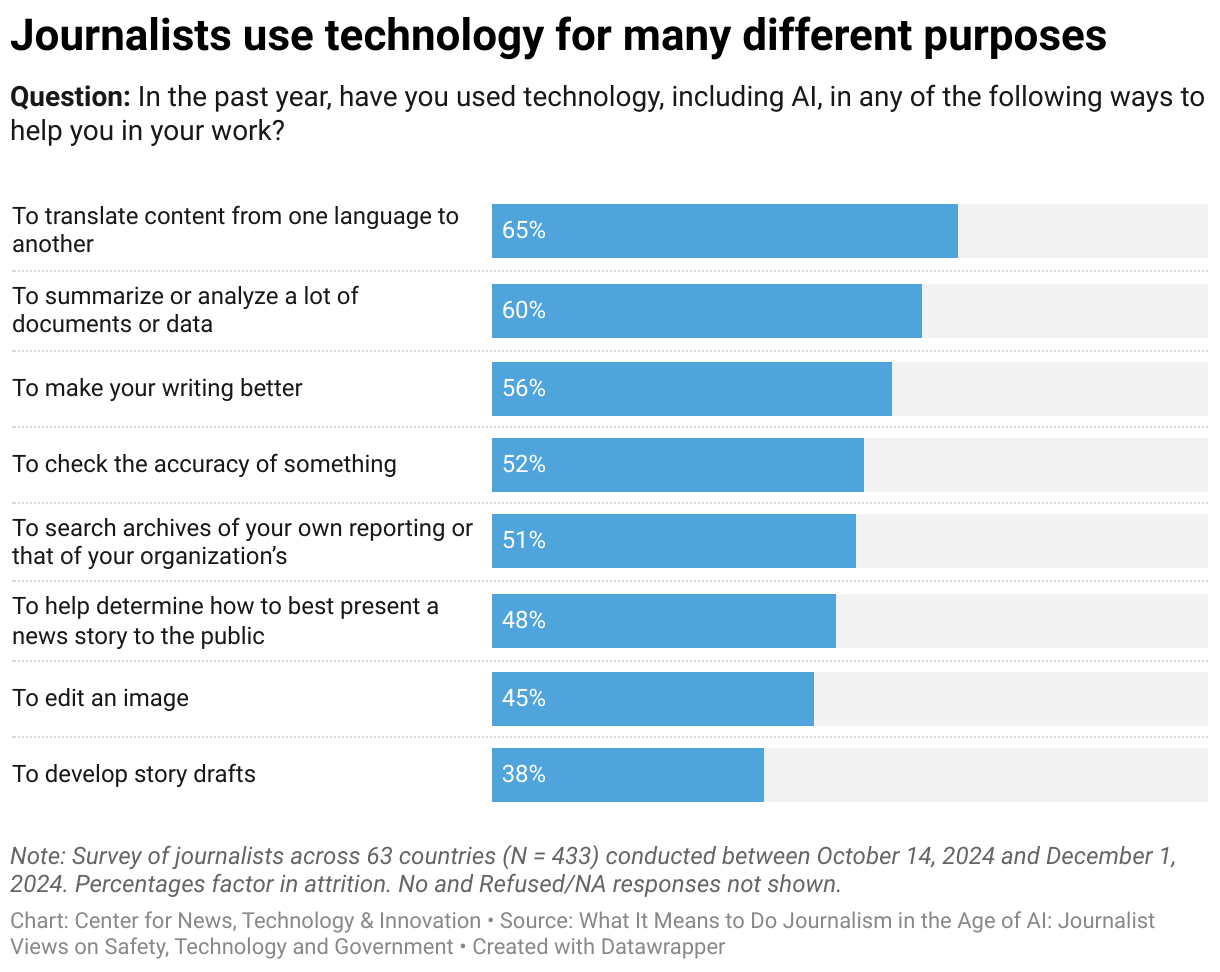
\includegraphics[width=\linewidth]{journalists-use-technology-for-many-different-purposes.png}
    \end{column}
    \begin{column}{0.48\textwidth} % Adjust width as needed
        \centering
        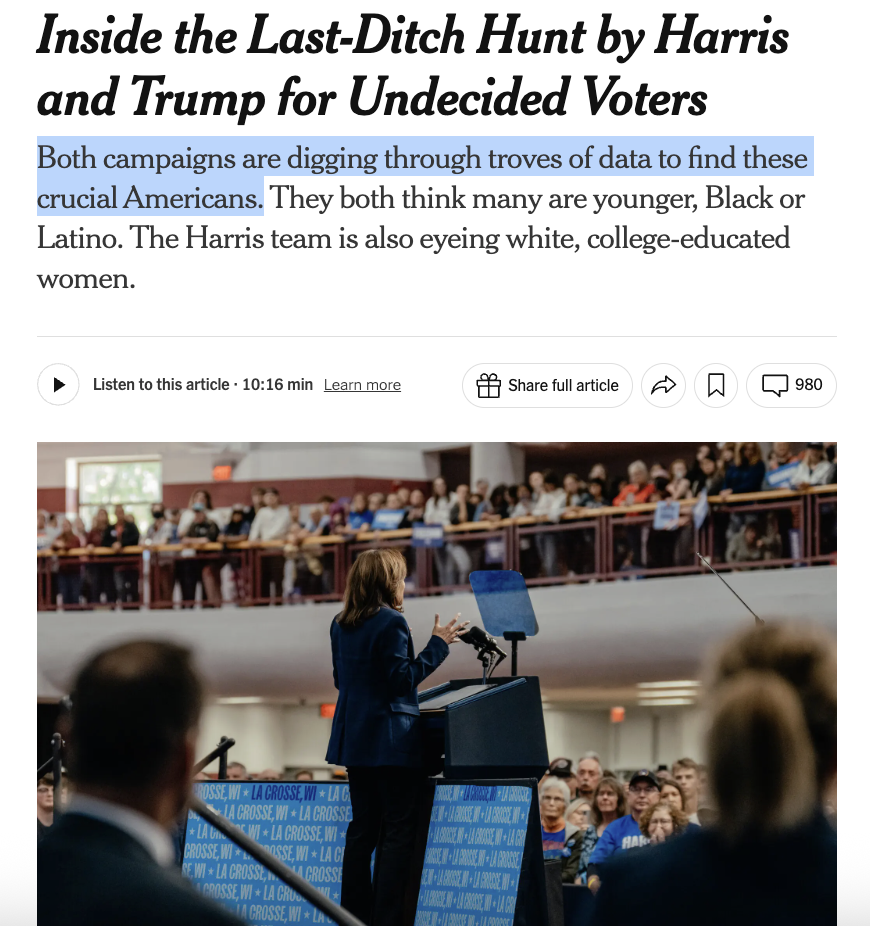
\includegraphics[width=\linewidth]{nyt_2024_campaigns_data.png}
    \end{column}
\end{columns}
}

%%%%%%%%%%%%%%%%%%%%%%%%%%%%%%%%%%%%%%%%%%%%%%%%%%%%%%%%%%%%%%%%%%
\frame{
    \frametitle{Chalabi: 3 Ways to Spot a Bad Statistic}
    \centering
    \href{https://www.ted.com/talks/mona_chalabi_3_ways_to_spot_a_bad_statistic}{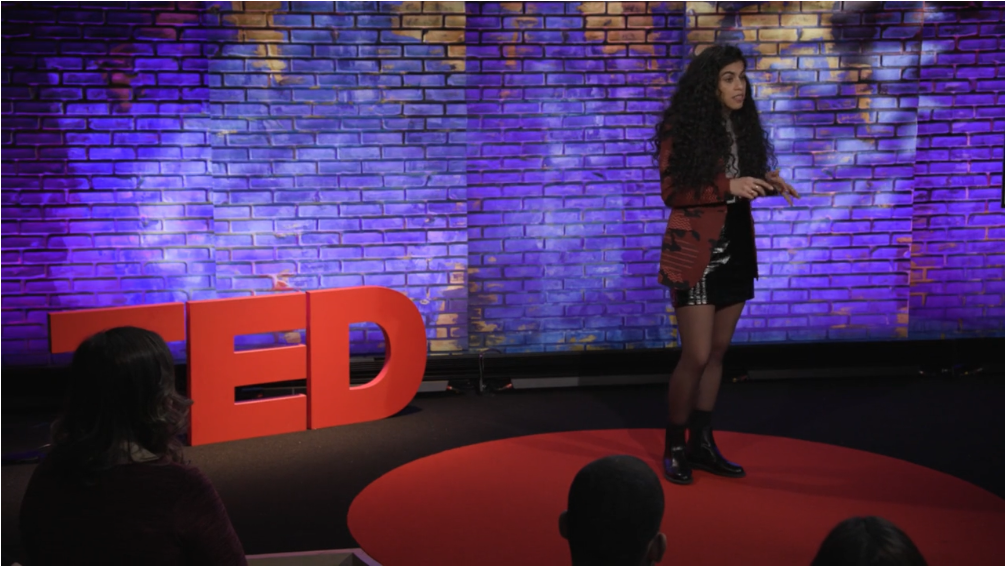
\includegraphics[height = .6\textheight]{chalabi-ted-talk.png}}
    
    \pause
    \begin{enumerate}
        \item Can you see uncertainty?
        \item Can we look beyond the averages?
        \item How was the data collected?
    \end{enumerate}
}

%%%%%%%%%%%%%%%%%%%%%%%%%%%%%%%%%%%%%%%%%%%%%%%%%%%%%%%%%%%%%%%%%%
\frame{
    \frametitle{Can you see the uncertainty?}
    \begin{itemize}[<+->]
        \item We rarely get a complete count of everything
        \item How do we know that the \textbf{sample} we choose is a good representative of the whole \textbf{population}?
        \item We will learn how to measure and communicate about the uncertainty inherent in statistics
        \item Humans do not do well with probability \\
            \only<5>{
                \begin{center}
                    \begin{minipage}{.8\textwidth}
                        \begin{block}{}
                            ``There are only five probabilities the average human can handle: 99 percent, one percent, 100 percent, zero, and 50-50. That's it.'' \\ - Richard Thaler, Nobel Laureate in Economics
                        \end{block}
                    \end{minipage}
                \end{center}
            }
            \only<6>{
                
\includegraphics[height = .35\textwidth]{dc_lottery.png}
            } 
            \only<7>{
                ~\\
                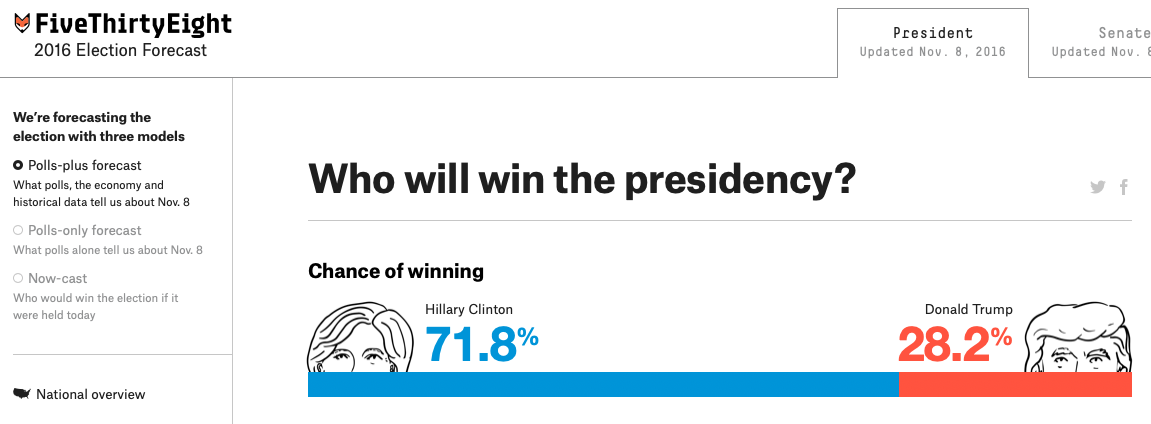
\includegraphics[height = .30\textwidth]{538_2016ElectionForecast.png}
            }
    \end{itemize}
}

%%%%%%%%%%%%%%%%%%%%%%%%%%%%%%%%%%%%%%%%%%%%%%%%%%%%%%%%%%%%%%%%%%
\frame{
    \frametitle{Can we look beyond the averages?}
    \only<1-2,4,6>{
        \begin{itemize}[<+->]
            \item There is always a trade-off between simplicity and precision when working with data
            \item We summarize data to make it easier to comprehend, but we may also lose important context
            \item<4,6> We will talk about using data visualization to communicate about data
            \item<6-> We will also talk about the importance of theory in understanding data, especially correlation vs. causation \\
            ~\\
            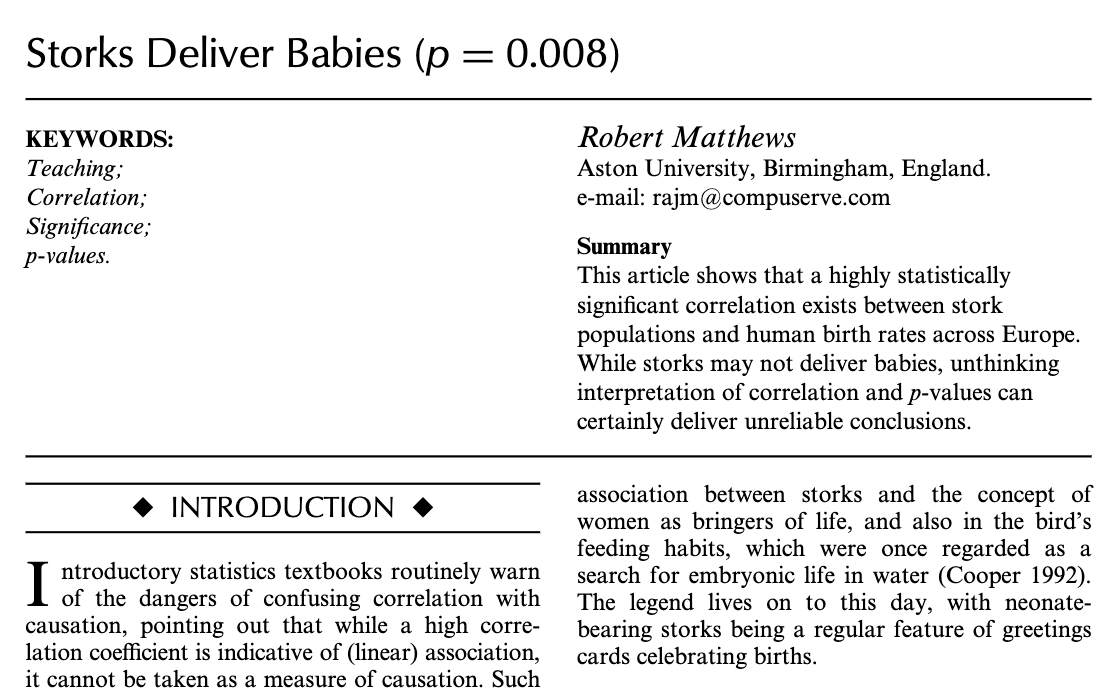
\includegraphics[height = .3\textheight]{storks.png}
        \end{itemize}
    }
    \only<3>{
        \centering
        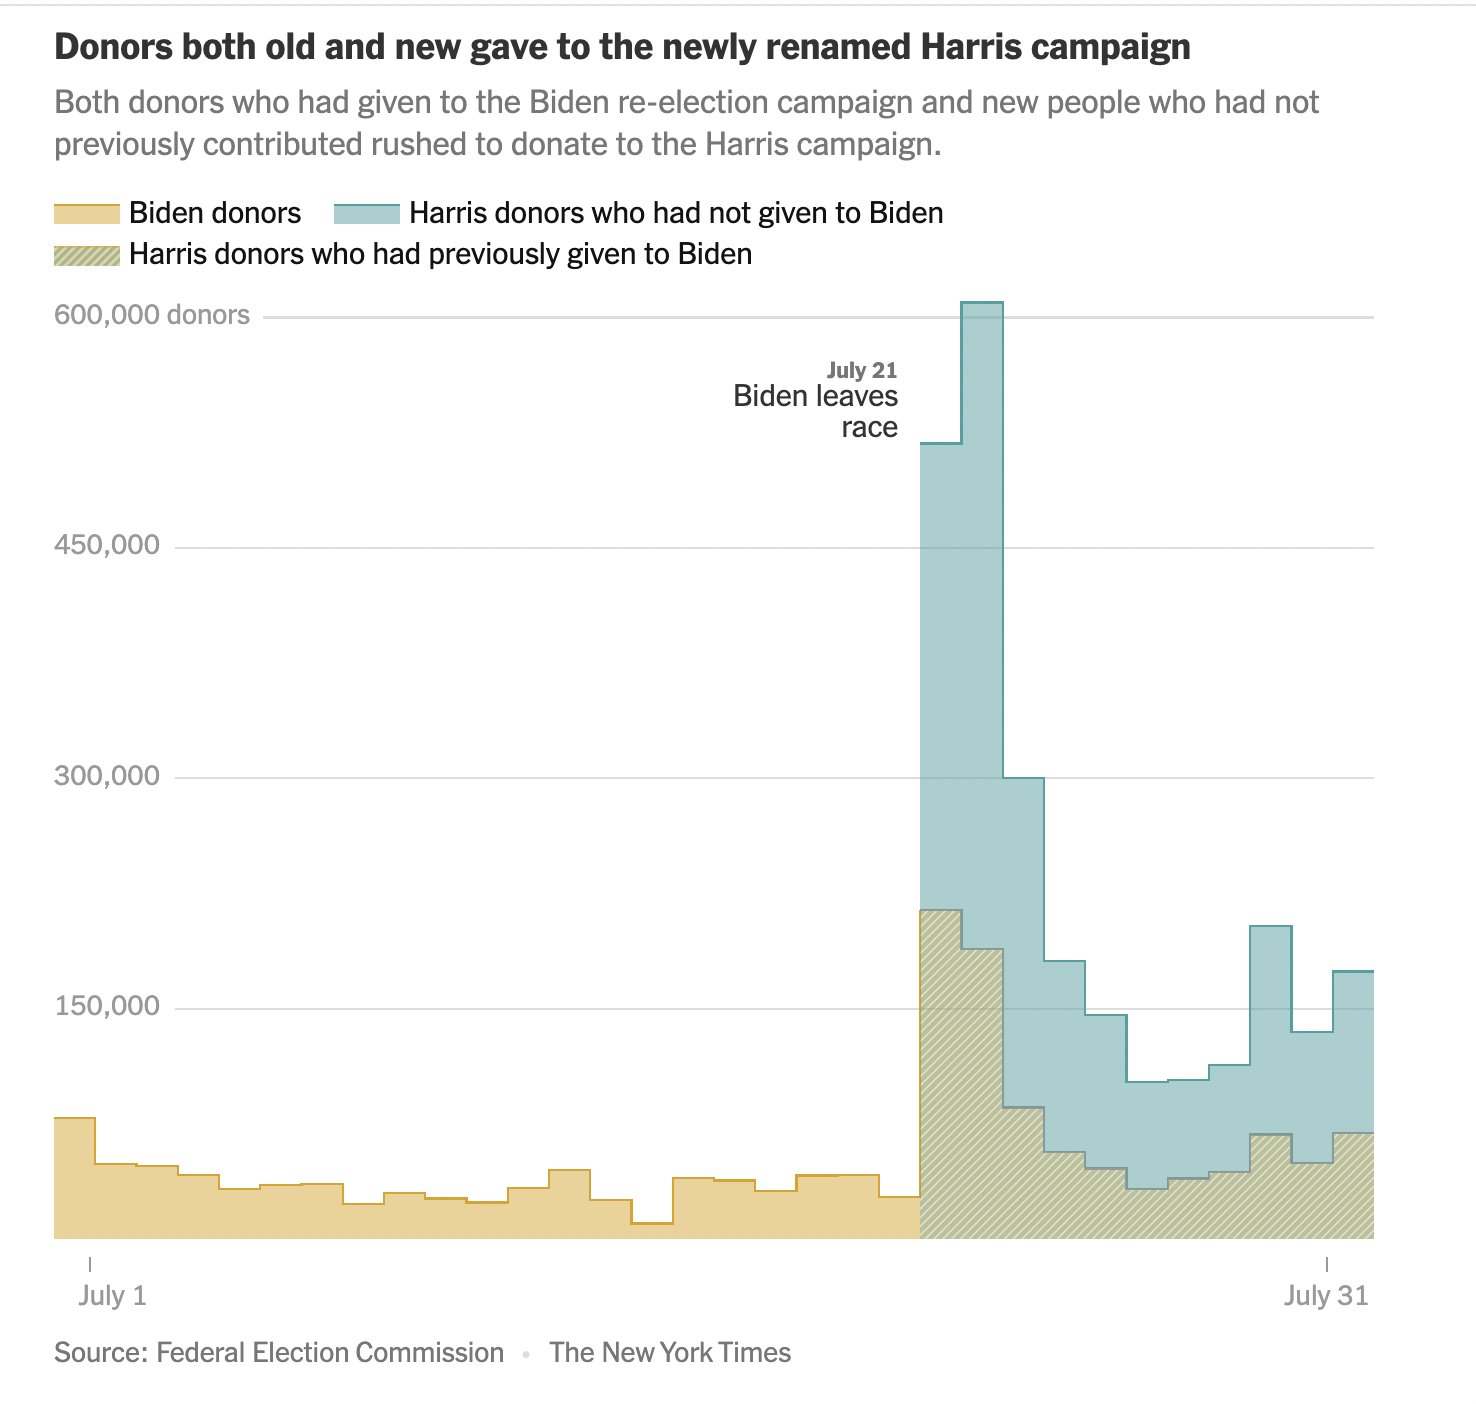
\includegraphics[height = .8\textheight]{harris_donors.jpeg}
    }
    \only<5>{
        \centering
        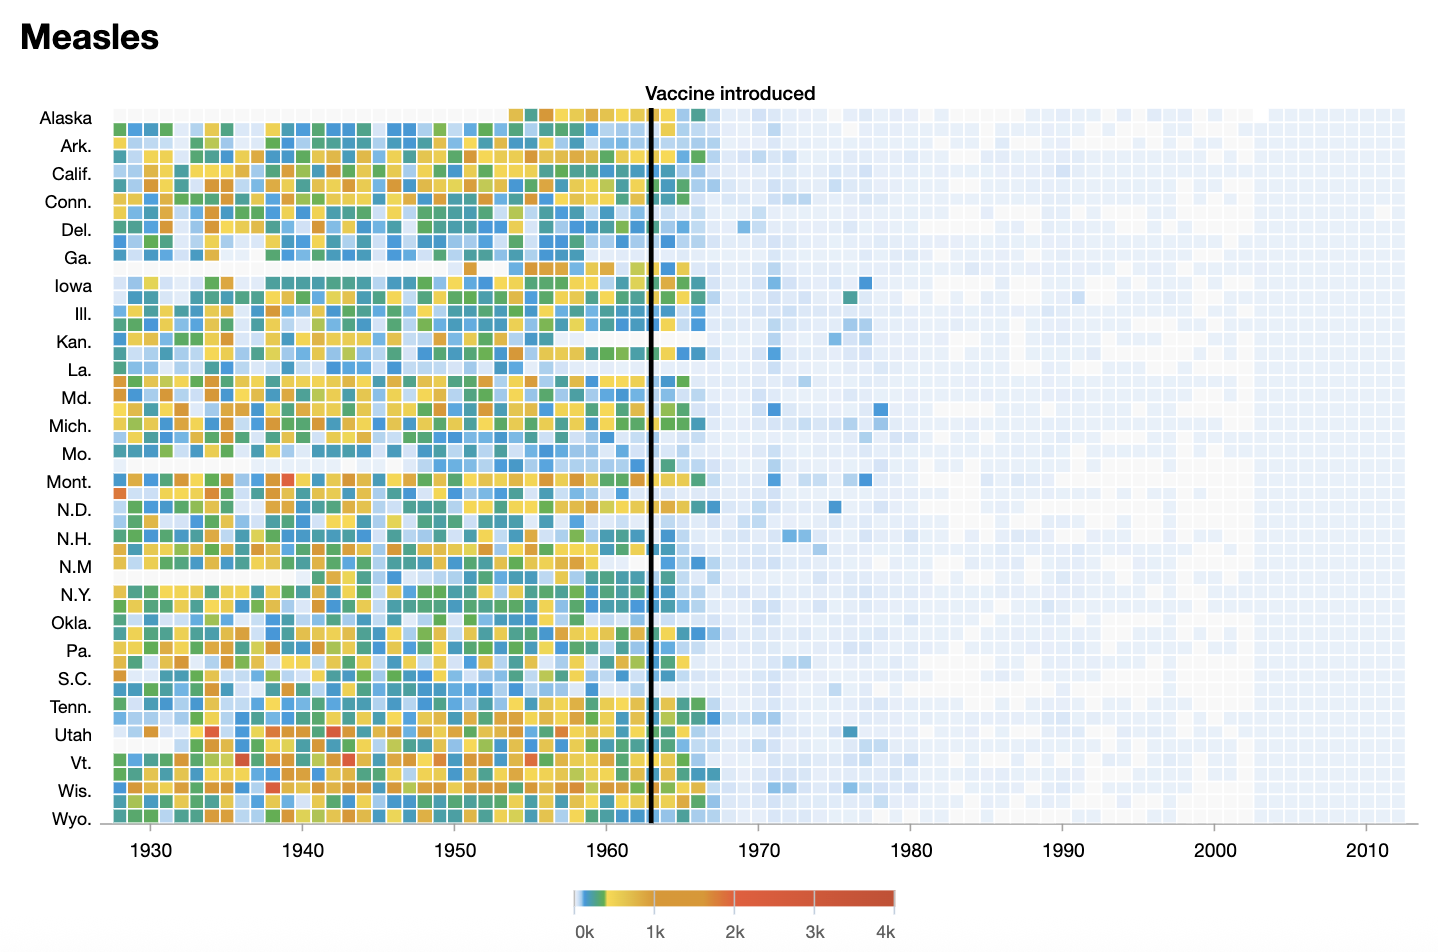
\includegraphics[height = .8\textheight]{wsj_measles_vaccine.png}
    }
}

%%%%%%%%%%%%%%%%%%%%%%%%%%%%%%%%%%%%%%%%%%%%%%%%%%%%%%%%%%%%%%%%%%
\frame{
    \frametitle{How was the data collected?}
    \only<1-4>{
        \begin{itemize}[<+->]
            \item<1-3> Data is not objective -- it is generated by humans
            \item<2-3> Some data is produced by unscrupulous actors \\
                \only<2>{~\\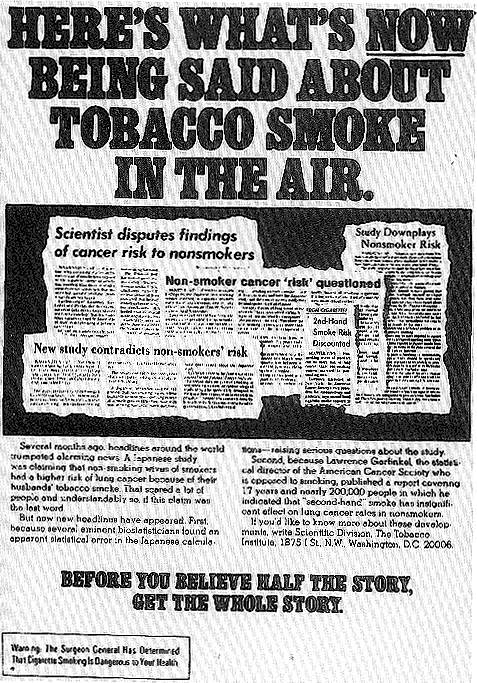
\includegraphics[height = .6\textheight]{tobacco_institute.png}}
            \item<3> But most of the time, poor analysis is not nefarious -- humans are imperfect
        \end{itemize}
    }
    \only<4-5, 7>{
        \begin{itemize}
            \item<4-> Garbage in = garbage out: no amount of statistical wizardry can compensate for bad data
            \item<5-> We will spend a lot of time thinking about the \textbf{data generating process} and how it can bias our results
            \item<7-> We will also discuss our ethical responsibilities around data
        \end{itemize}
    }
    \only<6>{
        \centering
        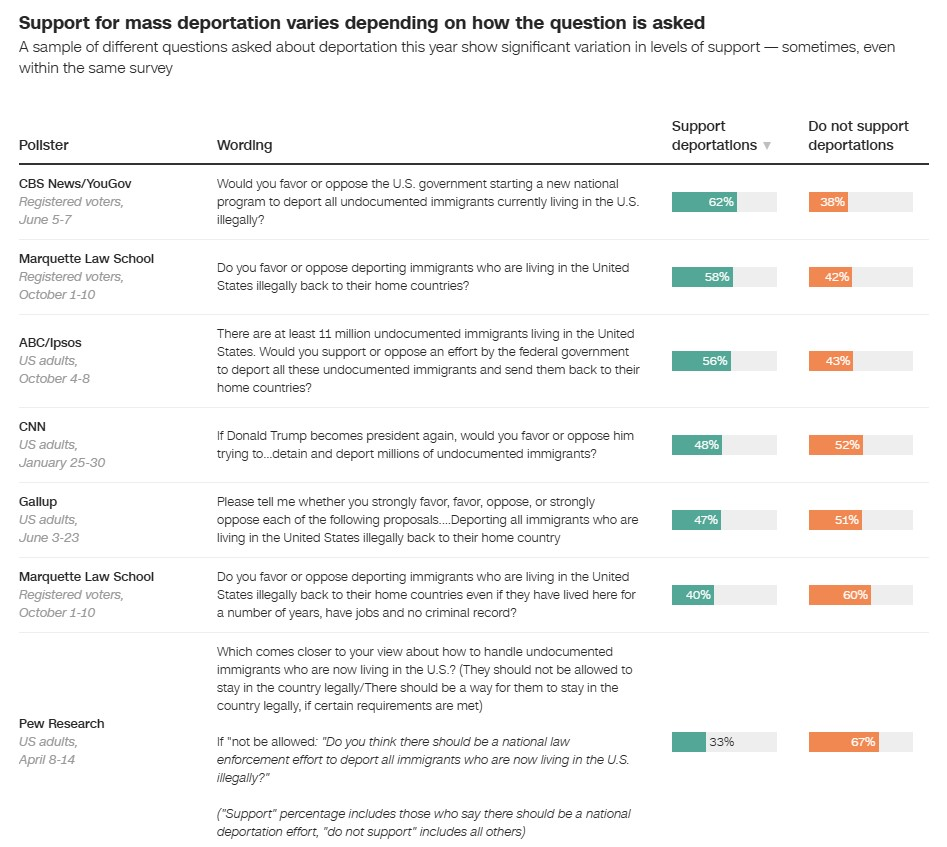
\includegraphics[height = .8\textheight]{poll_questions.jpeg}
    }
    \only<8>{
        \centering
        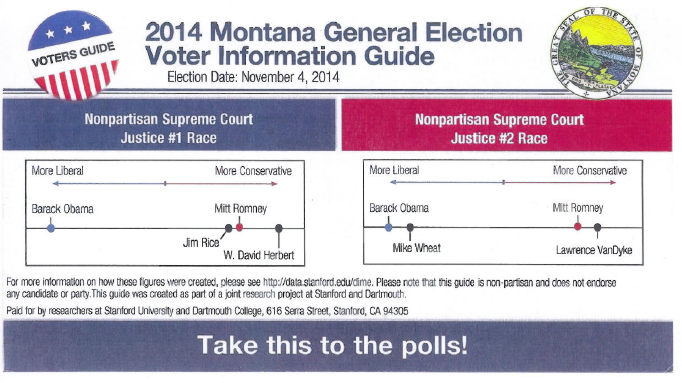
\includegraphics[width = .8\textwidth]{montana_experiment.png}
    }
}

%%%%%%%%%%%%%%%%%%%%%%%%%%%%%%%%%%%%%%%%%%%%%%%%%%%%%%%%%%%%%%%%%%
\frame{\frametitle{Group Discussion}

\only<1,3>{
    Introduce yourself to your neighbor(s) and take a few minutes to review these additional graphs from Mona Chalabi. Do any of these stand out to you as being good (or bad) examples of our three questions for spotting a bad statistic?
    
    \begin{enumerate}
        \item Can you see uncertainty?
        \item Can we look beyond the averages?
        \item How was the data collected?
    \end{enumerate}
}
\only<2> {
    \inserttimer{5}
}
}

%%%%%%%%%%%%%%%%%%%%%%%%%%%%%%%%%%%%%%%%%%%%%%%%%%%%%%%%%%%%%%%%%%

\frame{\frametitle{How the Course Will Work}

Your course grade is calculated as your grade on each of the following course components weighted by:
~\\
~\\
~\\
\begin{tabular}{l|l}
Attendance & 10\% \\
\hline
Lab assignments & 35\% \\
\hline
Class project & 20\% \\
\hline
Final exam & 35\% \\
\end{tabular}
}

%%%%%%%%%%%%%%%%%%%%%%%%%%%%%%%%%%%%%%%%%%%%%%%%%%%%%%%%%%%%%%%%%%

\frame{\frametitle{Lab Assignments}

\only<1-5>{
    \begin{itemize}[<+->]
        \item You will receive a very basic introduction to the R statistical programming language
        \item There are seven in-class Lab Days where you will work on an assignment applying the lessons learned in class to real-world problems using R
        \item You must watch the video lectures on R prior to the Lab Day class.
        \item You must turn in your completed lab assignment by 11:59pm the next day.
        \item You may complete these assignments on your own or in collaboration with other students. This means that you may work together to write code and/or solve problems. \textbf{Do not split up the questions or combine independent work.} Each student must submit an assignment on Blackboard.
    \end{itemize}
}
\only<6>{
    There is a software requirement for this course. Students may select from either option below.
    \vspace{1em}
    \begin{enumerate}
        \item \textbf{Option 1: Positron}. Positron is a free, open source development environment for R (and other coding languages) developed by the same creators of Posit Cloud.
        \item \textbf{Option 2: Posit Cloud}. Posit Cloud is a web-based version of the popular R development environment RStudio. At the time of this writing, a Student account for Posit Cloud costs \$5 per month.
    \end{enumerate}
}
}

%%%%%%%%%%%%%%%%%%%%%%%%%%%%%%%%%%%%%%%%%%%%%%%%%%%%%%%%%%%%%%%%%%

\frame{\frametitle{Piazza}
    \centering
    \href{https://piazza.com/gwu/fall2025/smpa2152}{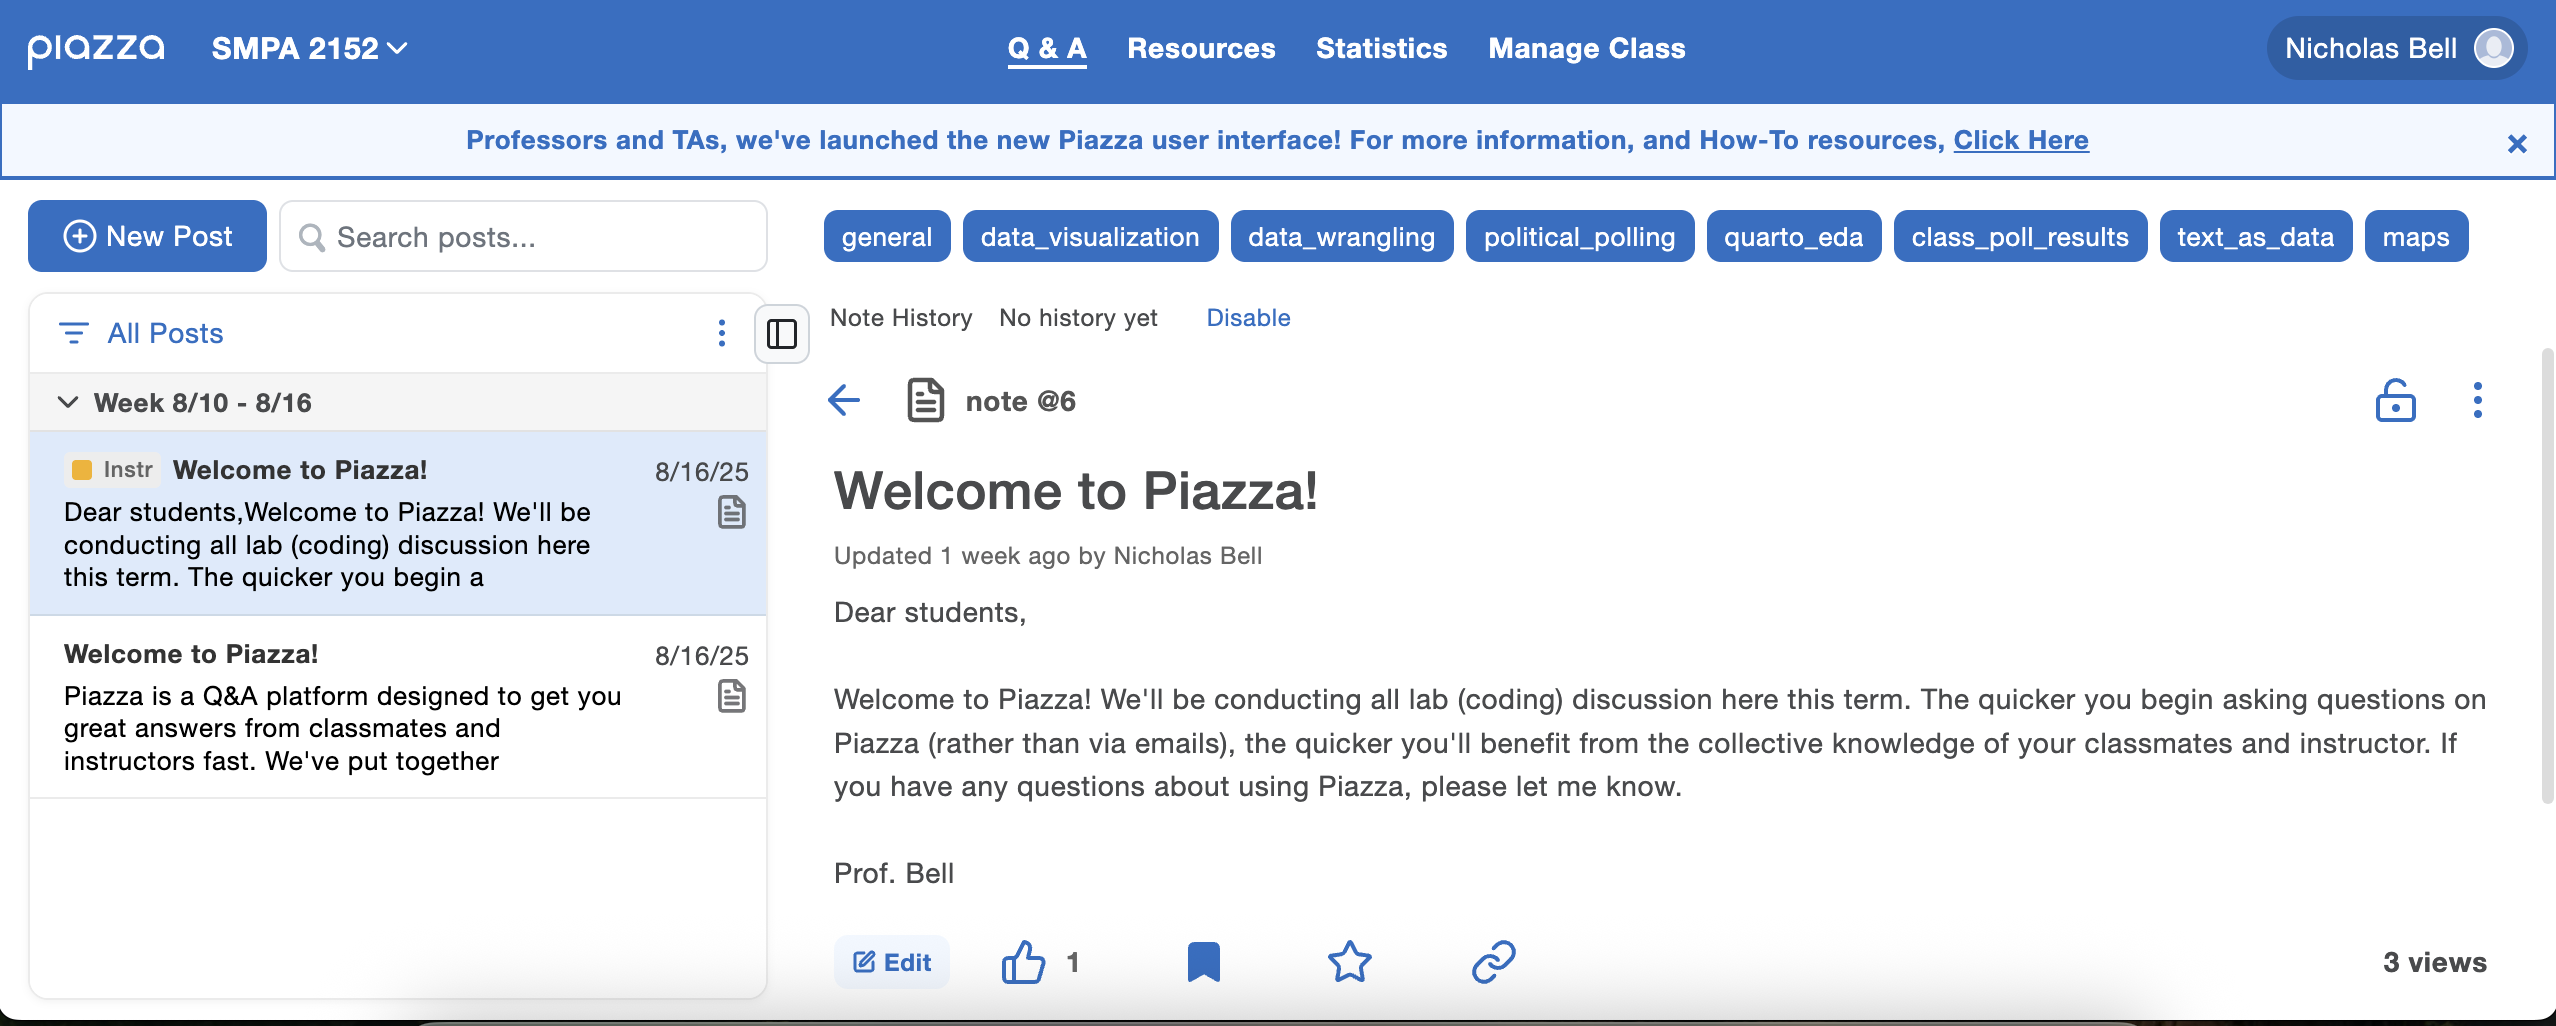
\includegraphics[width = .9\textwidth]{piazza.png}}
}

%%%%%%%%%%%%%%%%%%%%%%%%%%%%%%%%%%%%%%%%%%%%%%%%%%%%%%%%%%%%%%%%%%

\frame{\frametitle{Course Policy on Generative AI}

This course permits the use of Generative AI on \textbf{code} submitted for evaluation without restriction. However, the use of GAI tools for \textbf{written text} (e.g., exposition, analysis, etc.) is not permitted.
}

%%%%%%%%%%%%%%%%%%%%%%%%%%%%%%%%%%%%%%%%%%%%%%%%%%%%%%%%%%%%%%%%%%

\frame{\frametitle{Class Project}

\begin{itemize}[<+->]
    \item You will conduct a survey of your fellow GW students
    \item You will have an opportunity to indicate your preference for different roles in the survey process
    \item Your grade consists of your successful participation in the process plus a Lab Day assignment which uses the survey data you collect.
    \item You must complete the assigned CITI Ethics training to participate in the class project.
\end{itemize}
}

%%%%%%%%%%%%%%%%%%%%%%%%%%%%%%%%%%%%%%%%%%%%%%%%%%%%%%%%%%%%%%%%%%
\frame{
    \begin{center}
    \LARGE Questions?
    \end{center}
    ~\\
    ~\\
    \textit{\small Reminder: There is no class this Wednesday (prof. at a conference) or next Monday (Labor Day).}
}

%%%%%%%%%%%%%%%%%%%%%%%%%%%%%%%%%%%%%%%%%%%%%%%%%%%%%%%%%%%%%%%%%%
\frame{
    On your notecard, please write:
    \begin{enumerate}
        \item Preferred name
        \item Preferred pronouns
        \item Year in school and major
        \item Your background in coding and/or statistics
        \item One thing you hope to get out of this class
    \end{enumerate}
}

\end{document}
